\newpage
\subsection{Von der Bewegung}

\centerline{\textit{Maneuvering with an army is advantageous; with an undisciplined multitude, most dangerous.}}

%TODO: Skylining, Karte lesen, ...

Die Schlagkraft einer Truppe wird durch ihre Feuerkraft und ihre Mobilität bestimmt. Das Gelände zu kennen, es lesen zu können und sich korrekt sowohl alleine als auch im Trupp zu bewegen erfordert Kenntnis, Erfahrung und Übung. In diesem Abschnitt soll daher auf die Bewegung eingegangen werden.
\\ 

Grundsätzlich gilt, dass eine Bewegung von folgenden Faktoren bestimmt wird:
	\begin{itemize}
		\item Gelände -- Einen Bergkamm zu erreichen kann langwierig sein, und weitläufige freie Flächen sind zu meiden: eine Bewegung setzt eine 	entsprechende Vorkenntnis von Gelände und Erfahrung im Umgang mit der Karte voraus (siehe entsprechendes Kapitel).
		\item Trupp -- Je nach dem, welche Truppgröße und -zusammensetzung vorhanden ist, sind unterschiedliche Faktoren entscheidend: Tragen die Soldaten schwere oder leichte Lasten? Ist man zu viert oder sind es zwei Trupps die sich bewegen? Muss man Verwundete verlegen? 
		\item Verbündete Kräfte -- Befinden sich verbündete Truppen oder Fahrzeuge in der Nähe, welche Platz zum Manövieren benötigen? Zu dicht gedrängte Formationen laden zu Beschuss durch Artillerie ein -- stehe ich zu dicht an meinen Kameraden? Sichere ich in die richtige Richtung? Sichern wir in alle Richtungen?
		\item Feindliche Kräfte -- Welche feindlichen Kräfte sind wo zu erwarten? Wurden sie aufgeklärt, oder ist man sich unsicher wer das Territorium hält?
		\item Ziel der Bewegung -- Keine Bewegung ohne Ziel! Wo soll es hingehen? Was ist der Auftrag dort? Welcher Zeitrahmen steht zur Verfügung?
	\end{itemize}
Egal ob man nun über ein Stoppelfeld zur nächsten Deckung hetzt, sich langsam durch eine Siedlung arbeitet oder in eine Stellung am Waldrand gleitet: es gibt Grundregel und Dinge, die jeder Soldat wissen sollte. Dazu gehören Bewegungsarten, Formationen und grundsätzliches zum Umgang mit der Waffe während der Bewegung.

\subsubsection{Bewegungsarten}

Man unterscheidet zwischen folgenden Bewegungsarten:
	\begin{itemize}
		\item Gleiten -- Tiefste Forstbewegungsart, das Kriechen. Geschieht meist langsam um sich anzuschleichen oder eine extrem flache Silhouette zu bieten.
		\item Geduckt -- Schneller als das Gleiten, ermüdet den Soldaten rasch und passiert meist intuitiv während Bewegung hinter Deckung.
		\item Gehen -- Aufrechtes Gehen, typische Bewegungsart wenn längere Strecken überbrückt werden müssen
		\item Sprung -- Schnelles Rennen, meist zur nächsten Deckung oder um eine Distanz schnell zu überbrücken
	\end{itemize}

\subsubsection{Die Formationen}

	Zur Bewegung durch das Gelände verwendet man Formationen, welche der sich bewegenden Gruppe Vor- und Nachteile bieten. Sie sollten jederzeit dem Gelände sowie erwarteten oder bekannten Feindkräften angepasst werden. Die Formationen welche im TTT Verwendung finden sind der \textit{Stack}, die \textit{Kolonne} und die \textit{Schützenkette}. 

\paragraph{Der Stack}$\ $\\

	Der Stack ist die Sammelformation vor dem Abmarsch und als Bewegungsformation beim Einstieg in Fahrzeuge. Zudem dient er als Formation für den direkten Zugriff in Räume (siehe dazu CQB \autoref{CQB}). Grundsätzlich wird der Stack in den klassischen (engen) <<Stack>> und <<Stack weit>> unterteilt. Beim <<Stack weit>> werden die Abstände lediglich erweitert.\\
	\begin{figure}[!htb]
		\centering
		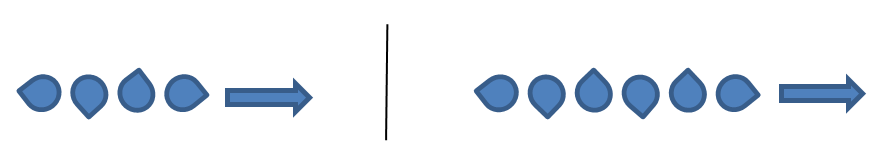
\includegraphics[width=15cm]{./Grafiken/Abschnitt/Stack.png}
		\caption{Stack 4 und 6 Mann}
	\end{figure}

\paragraph{Die Kolonne}$\ $\\

	Die Kolonne dient als Formation im offenen Gelände und ist die Standardformation für den Marsch. Hierbei muss man zwischer einer Besonderheit im \ac{TTT} der Buddy - Kolonne und der klassischen Kolonne unterscheiden. Die Buddy - Kolonne garantiert, dass beispielsweise MG-Schütze und MG-Assistent immer zusammenbleiben, zudem verringern sie die Ausfallzahl, da sich Buddys besser gegenseitig unterstützen können. Im Gegenzug ist die klassische Kolonne weniger anfällig für Sprengsätze und Beschuss. Die Abstände zwischen den Teams sollten etwa 20 m betragen.\\
		\begin{minipage}[t]{1\textwidth}
			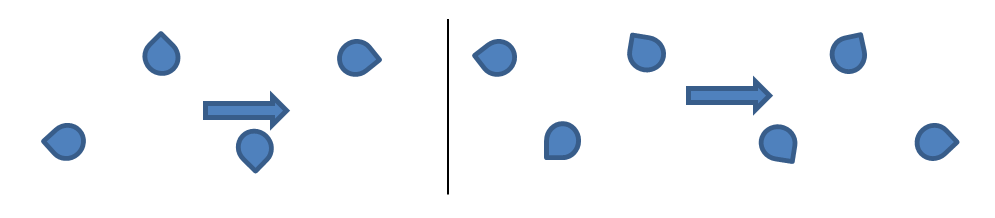
\includegraphics[width=13cm]{./Grafiken/Abschnitt/Kolonne.png}
			\label{Kolonne}
		\end{minipage}
		\begin{minipage}[t]{1\textwidth}
			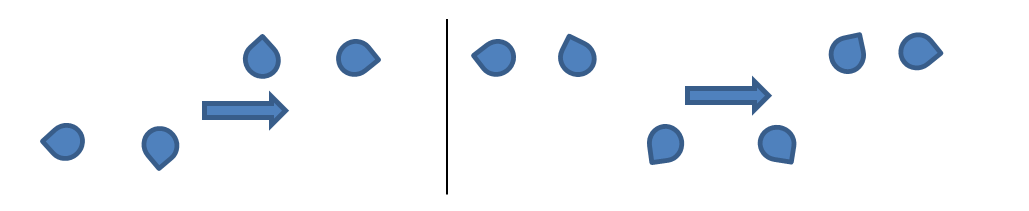
\includegraphics[width=13cm]{./Grafiken/Abschnitt/Buddykolonne.png}
		\end{minipage}

\paragraph{Die Schützenkette}$\ $\\

	Die Schützenkette ist eine Formation, die zum Bezug der Stellung, in Deckung an Mauern und -- in Ausnahmefällen! -- zum Anmarsch auf einen Feind benutzen. Sie bietet maximale Feuerkraft in vermuteter Feindrichtung, lässt jedoch die Flanken und den Rückraum ungesichert. Die Schützenkette kann effizienter gestaltet werden durch entsprechende Flanken- und Rücksicherung.\\
		\begin{minipage}[t]{1\textwidth}
			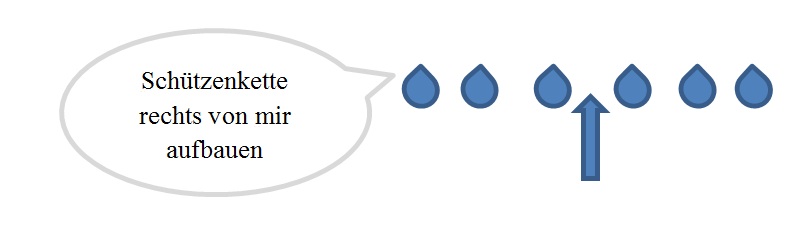
\includegraphics[width=13cm]{./Grafiken/Abschnitt/Schuetzenkette1.png}
		\end{minipage}
		\begin{minipage}[t]{1\textwidth}
			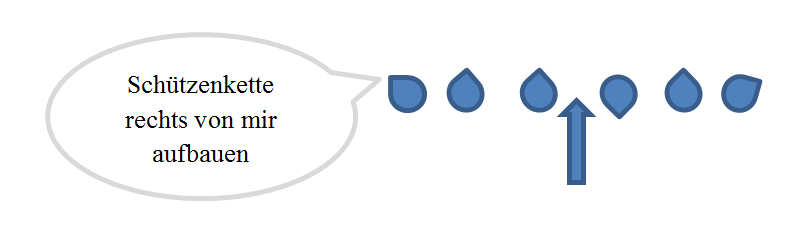
\includegraphics[width=13cm]{./Grafiken/Abschnitt/Schuetzenkette2.png}
		\end{minipage}

\subsubsection{Sicherungsbereiche}

Während der Bewegung hat jedes Mitglied eines Trupps in eine bestimmte Richtung zu sichern. Dabei gelten für den 4-Mann-Trupp folgende Sicherungsbereiche:
	\begin{itemize}
		\item Nr.1 sichert auf 12 Uhr 
		\item Nr.2 sichert auf 9 Uhr 
		\item Nr.3 sichert auf 3 Uhr 
		\item Nr.4 sichert auf 6 Uhr 
	\end{itemize}
Und für den 6-Mann-Trupp:
	\begin{itemize}
		\item Nr.1 sichert auf 12 Uhr 
		\item Nr.2 sichert auf 10 Uhr 
		\item Nr.3 sichert auf 2 Uhr 
		\item Nr.4 sichert auf 4 Uhr 
		\item Nr.5 sichert auf 8 Uhr
		\item Nr.6 sichert auf 6 Uhr 
	\end{itemize}

\subsubsection{Umgang mit der Waffe}

Ständig bereit zu sein, ein Feuergefecht aufzunehmen kann aus mehreren Gründen unpraktisch oder sogar gefährlich sein. Daher gilt grundsätzlich die Waffe während des Marsches herunterzunehmen und erst in den Anschlag zu nehmen, wenn eine von folgenden Bedingungen zutrifft:
	\begin{itemize}
		\item Es muss ein erkannter Feind bekämpft werden.
		\item Die Waffe muss eingewiesen werden oder die Optik soll zur Aufklärung genutzt werden.
		\item Feindliche Kräfte auf Tuchfühlung (im Umkreis von 10m)
		\item Es wurde liegend oder stehend eine Stellung bezogen oder Sicherungsbereiche benannt.
	\end{itemize}

In allen anderen Fällen ist die Waffe unten zu halten. In einer Basis ist sie zudem zu \textit{sichern}! \\

Die Waffe gesenkt zu haben hat zahlreiche Vorteile:
	\begin{itemize}
		\item Das Sichtfeld ist deutlich größer.
		\item Die Wahrscheinlichkeit von Beschuss eigener Kräfte und dem Verraten der Position durch versehentliches Abfeuern der Waffe ist geringer.
		\item Die Ausdauer leidet weniger und man bewegt sich schneller.
	\end{itemize}
Die Waffe erhoben zu haben hat einige Nachteile:
	\begin{itemize}
		\item Entwicklung eines Tunnelblicks: Der Träger blickt nur noch in eine Richtung (meist vorn und eventuell sogar noch durch die Optik)
		\item Der Soldat bewegt sich langsamer und ermüdet schneller
		\item Der Soldat gefährdet eigene Kameraden!
	\end{itemize}
Es gilt zudem, das \textit{unter keinen Umständen} die Waffe auf eigene Kräfte gerichtet werden!

\paragraph{Kreuzen}$\ $\\
	Unter \textit{Kreuzen} versteht man das Queren oder Kreuzen einer Feuerlinie eines Kameraden. Wo immer möglich ist dies zu vermeiden. Das gilt ganz besonders für Fahrzeuge, dort ist auch eine mögliche Bewegungsrichtung (nach vorn / nach hinten) jederzeit frei zu halten. Es hilft ungemein, bereits sofort nach dem Beziehen einer Stellung zu überprüfen, ob die Kameraden immer noch entsprechend manövrieren können. Wann immer man doch Kreuzen muss, ist dies verbal und früh genug anzukündigen: \textbf{"Achtung, ich kreuze!"}

\paragraph{Annäherung an eigene oder verbündete Kräfte}$\ $\\

Um sich an befreundete Truppen anzunähern, sollten diese möglichst durch Funk und durch persönliche Ansprache (ähnlich dem Kreuzen) gewarnt werden. Idealerweise gibt man die Annäherungsrichtung mit dazu an.\\

\subsubsection{Vokabular der Bewegung}
\begin{longtable}{| >{\columncolor{backcolor}}l | p{13cm} |}
	\caption[Vokabular Bewegung]{Begriffe der Bewegung} \\
	\hline
	\textbf{Begriff} & \textbf{Bedeutung} \\
	\hline
	Bereitmachen zum Sprung / Bereit zum Sprung & \\
	\hline
	Sprung auf, Marsch Marsch! & \\
	\hline
	Verschieben & \\
	\hline
	Verlegen & Bewegen über eine lange Strecke \\
	\hline
	Ausweichen & Lösen von feindlichen Kräften, meist Rückzug zu besser zu verteidigenden Position, oft mit Ablenkungen oder Deckungsfeuer kombiniert.\\
	\hline
\end{longtable}